\chapter{Configuring Advanced Networking}

\section{Networking Basics Resumed}
\subsection{Network configuration tools}
\begin{tabular}{rM{0.68}}
	\toprule
	\textbf{Terms} &\textbf{Description} \\
	\midrule
	\textbf{ip addr show}	&Shows address information about all network interfaces.\\
	\midrule
	\textbf{ip -s link show ens33}	&Shows statistics about packets but for interface \verb|ens33|. Same as \verb|ip -s link|, but for a specific interface. \\
	\midrule
	\textbf{ip route}	&Shows routing information\\
	\midrule
	\textbf{traceroute / tracepath}	&For analysing a particular route or path.\\
	\midrule
	\textbf{netstat / ss}	&Analyse ports and services currently listening for incoming connections.\\
	\bottomrule
\end{tabular}

\subsection{Network Manager}
\textbf{NetworkManager} is used to both manage and monitor network settings. While the settings made with the IP tool act directly on the NICs, they're temporary and wiped with every boot or even bringing the interface down and up again. The network manager uses config scripts in \verb|/etc/sysconfig/network-scripts| to store our configs and use them after every boot. The settings can be managed using either \verb|nmcli| or \verb|nmtui|. The former is preferred for scripts while \verb|nmtui| is preferred for manual configs. 

\subsubsection{nmcli concepts}
\begin{itemize}
	\item A \textbf{device} or an \textbf{interface} is a network interface, corresponding to the hardware NIC (Network Interface Card). 
	\item A \textbf{connection} is a collection of configuration settings for a \textit{device}. 
	\item Multiple connections can exist for the same device, but since they operate on the same settings for the device, only one of them can be active. 
	\item All the connections (and some details) can be shown with the command \verb|nmcli con show|. 
	\item To show all the details for a particular connection, we have to use the command \verb|nmcli con show <interface name>| like \verb|nmcli con show wlo1| (where \textit{wlo1} is the name of the connection).
	\item To see the connection status for a device, we use \verb|nmcli dev status|. This shows us which devices are connected and which connection they're presently using. 
	\item To see the details of the actual NIC device, we use \verb|nmcli dev show <deviceName>|.
\end{itemize}

\subsection{Creating Network Interfaces with nmcli}
\vspace{-10pt}
To add a new connection using \verb|nmcli| that has the name \textit{dhcp} that auto-connects using dynamic IP on interface \textit{eno1}, we use:

\vspace{-15pt}
\begin{minted}{console}
# nmcli con add con-name "dhcp" type ethernet ifname eno1 
\end{minted}
\vspace{-10pt}	

\noindent
To add a new connection \textit{static} that uses a static ip that doesn't connect automatically, we use:

\vspace{-15pt}
\begin{minted}{console}
# nmcli con add con-name "static" type ethernet ifname eno1 autoconnect no ip4 192.168.122.102 gw4 192.168.122.1
\end{minted}
\vspace{-10pt}	

\noindent
Now, the available connections can be checked with \verb|nmcli dev status|. The we can connect the \textit{static} connection using \verb|nmcli con up static| and then switch back to the original connection \textit{dhcp} using \verb|nmcli con up dhcp|.

\subsection{Modifying Network Interfaces using nmcli}

To see the details of the \textit{static} connection, we use \verb|nmcli con show static|. Then, to add/modify the DNS server address for that connection, we use the \verb|con mod| keywords, which makes the command:

\vspace{-15pt}
\begin{minted}{console}
# nmcli con mod "static" ipv4.dns 192.168.122.1
\end{minted}
\vspace{-10pt}	

\noindent
Note that the modification requires the \verb|ipv4| keyword instead \verb|ip4|. To define a second IPv4 DNS for the \textit{static} connection, we use the \verb|+| symbol to denote that a new value for the item should be added and the old value shouldn't be overwritten. The command then becomes: 

\vspace{-15pt}
\begin{minted}{console}
# nmcli con mod "static" +ipv4.dns 8.8.8.8
\end{minted}
\vspace{-10pt}	

\noindent
An existing static IP address and gateway can be edited using:

\vspace{-15pt}
\begin{minted}{console}
# nmcli con mod "static" ipv4.addresses "192.168.100.10/24 192.168.100.1"
\end{minted}
\vspace{-10pt}	

\noindent
A secondary IPv4 address can be added using:

\vspace{-15pt}
\begin{minted}{console}
# nmcli con mod "static" +ipv4.addresses "10.0.0.10/24"
\end{minted}
\vspace{-10pt}	

\noindent
Finally, to activate all the above settings, we use: \verb|nmcli con up static|.

\subsection{Working directly with Configuration Files}
All the \verb|nmcli| tool really does while adding or modifying settings is write the changes to the configuration files in \verb|/etc/sysconfig/network-scripts/ifcfg-<interfaceName>|. We may choose to edit them directly if needed. Then, after making the necessary modifications, we ask the NetworkManager service to reload the configuration using \verb|nmcli con reload|.

\subsection{Managing Hostname and DNS}
The hostname is stored in the file \verb|/etc/hostname| and can be edited directly or using the \verb|hostnamectl set-hostname <newHostName>| command. The current hostname can then be viewed using \verb|hostnamectl status|.

The value of the search domain and preferred nameserver (i.e., the one that the NetworkManager uses by default) is auto-pushed from \verb|/etc/sysconfif/network-scripts/|\\\verb|ifcfg-<connectionName>| to the file \verb|/etc/resolv.conf|. 

\section{Understanding Routing}
Let us consider the following network:

\begin{figure}[H]
	\centering
	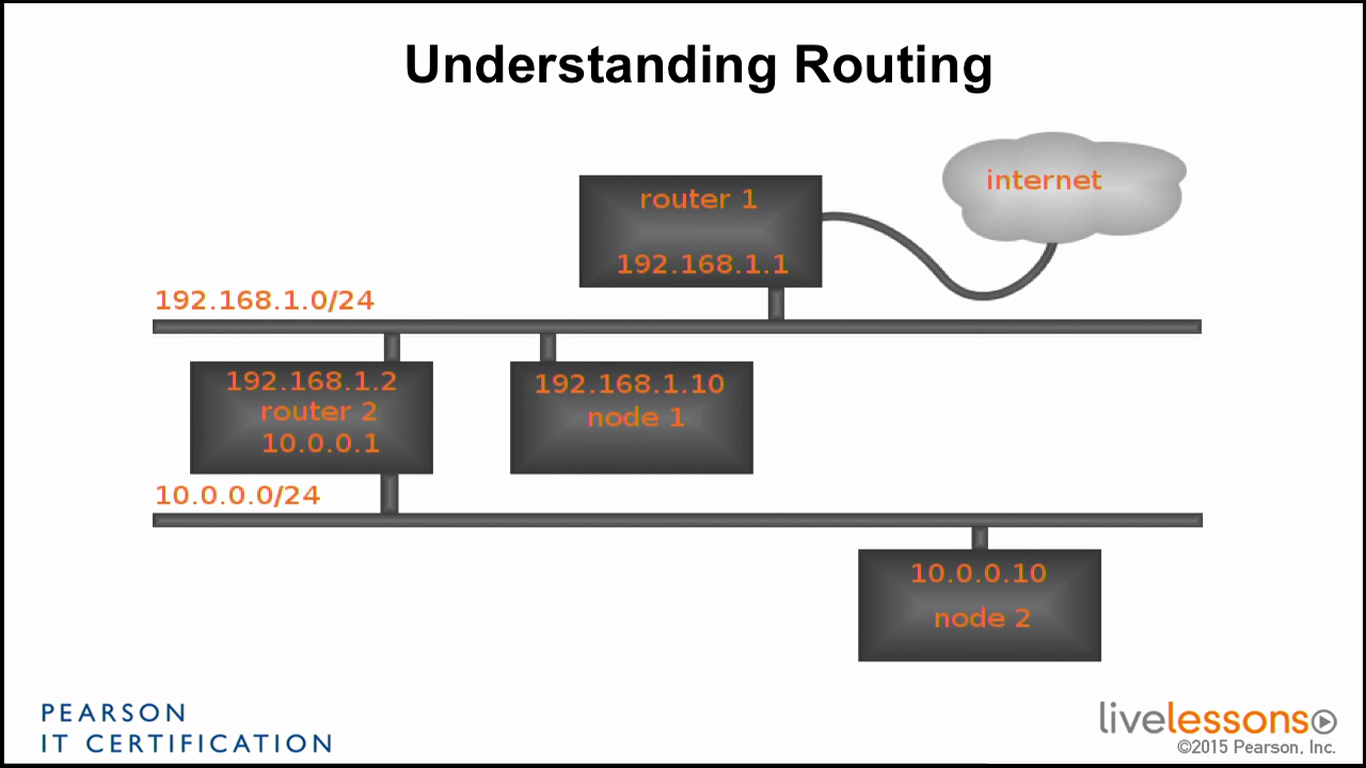
\includegraphics[width=0.9\linewidth]{Mod2/chapters/2.6.a}
	\caption{Sample Network}
	\label{fig:2}
\end{figure}

\noindent
Here, we see two different networks - the \verb|10.0.0.0/24| network connected to the inner \verb|192.168.1.0/24| network via \textit{router 2} (\verb|10.0.0.1|), which in turn connects to the internet via the edge router with IP \verb|192.168.1.1| - \textit{router 1}. 

For any packet headed to the internet on network 2, i.e., any packet originating from \textit{node 2}, the default gateway will have to be \textit{router 2} (\verb|10.0.0.1|). This gets the packet on to the \verb|192.168.1.0/24| network, where the default gateway is \textit{router 1} (\verb|192.168.1.1|), which passes it on to the internet. 

However, when the packets originate from node 1 (\verb|192.168.1.10|), there are two possible routes - if the packet is destined for the \verb|10.0.0.0/24| network, then the gateway should be \textit{router 2} (\verb|192.168.1.2|). But if the packet is for any other network, then the default gateway of \textit{router 1} (\verb|192.168.1.1|) should be used. Thus, a static route should be defined on node 1 for the \verb|10.0.0.0/24| network. 

\section{Setting up Static Routing}
The most convenient way to set up static routes is to use \verb|nmtui|. Let's assume we're setting up static routing for node 2 in our last example.

\begin{figure}[H]
	\centering
	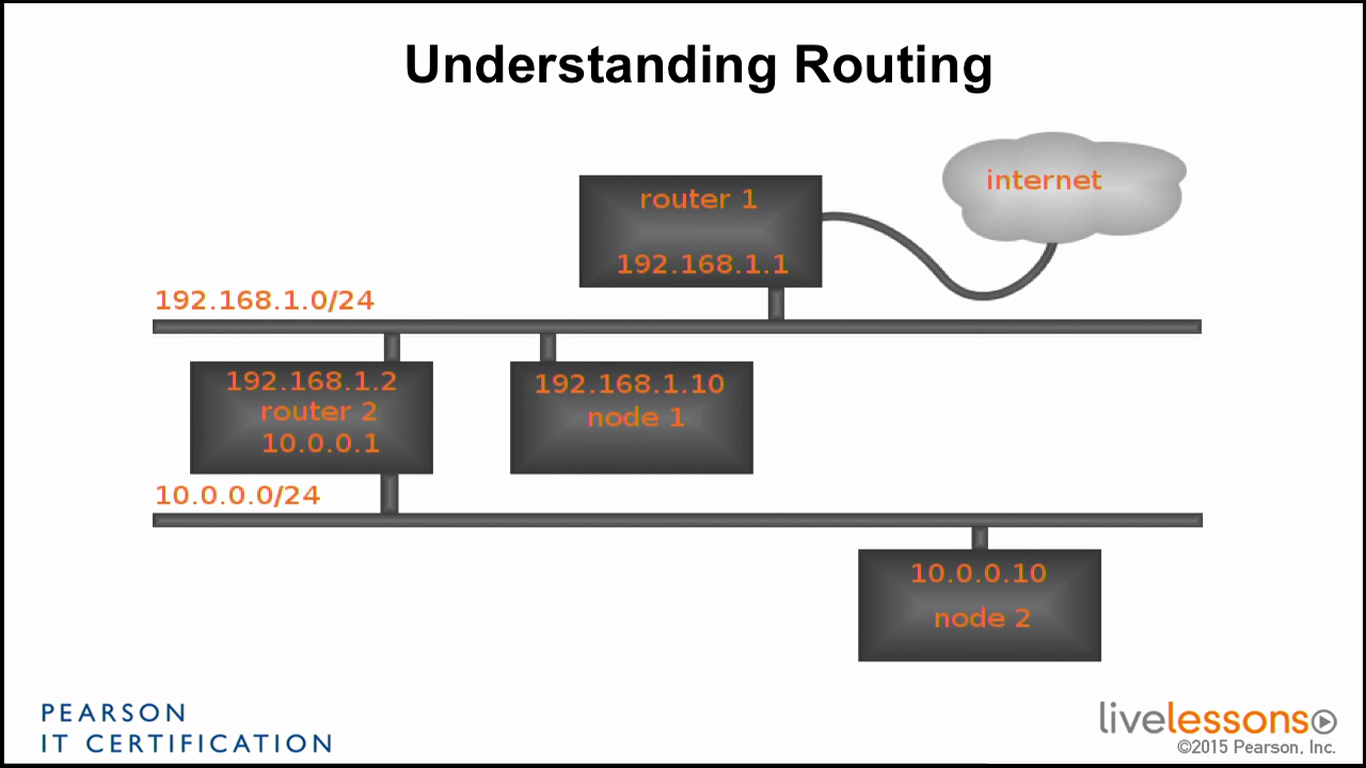
\includegraphics[width=0.9\linewidth]{Mod2/chapters/2.6.a}
	\caption{Network Diagram}
	\label{fig:2}
\end{figure}	

We need to edit the existing connection to include the new static route. For this, we select the options: \verb|Edit a Connection| $\rightarrow$ Select the connection to use $\rightarrow$ \verb|Edit...| $\rightarrow$ \verb|Routing| section $\rightarrow$ \verb|Edit...| $\rightarrow$ \verb|Add...| $\rightarrow$ Type the address of the network for which the static route will be defined in \verb|Destination/Prefix| (with the Network ID and prefix, like, \verb|10.0.0.0/24|) $\rightarrow$ Add the IP address of the router that leads to the network in the \verb|Next Hop| section (\verb|192.168.1.2| in our case). 

The \textbf{metric} of the connection is how a router chooses which route to take when there are multiple routes available to another network. Thus, it's only useful when there are multiple routes available for the same network, and is irrelevant to us right now. We now choose \verb|<Ok>| $\rightarrow$ \verb|<Ok>| $\rightarrow$ \verb|<Quit>|. 

Note however, that the new route won't be added to the network configuration till either the connection is \textit{refreshed} (by reactivating the connection) or the NetworkManager service is restarted. We could do this by \verb|nmtui| $\rightarrow$ \verb|Activate a Connection| $\rightarrow$ Select the connection which we edited $\rightarrow$ \verb|Activate|. Now the output of \verb|ip route show| will show the static route as well. 

If the interface name was \textit{ens33}, The \verb|/etc/sysconfig/network-scripts| directory now has a new file called : \verb|route-ens33| with the following contents:

\vspace{-15pt}
\begin{minted}{bash}
ADDRESS0=10.0.0.0
NETMASK0=255.255.255.0
GATEWAY0=192.168.1.2
\end{minted}
\vspace{-10pt}	

\noindent
Note that the nmtui utility has translated the \verb|/24| prefix from the \textbf{CIDR} (Classless Inter-Domain Routing) notation \verb|10.0.0.0/24| to the standard Network IP and Network Masks, where \verb|/24| translates to the network mask of \verb|255.255.255.0|. 

	\section{Understanding Network Bridges}
A network bridge is a device that connects two or more networks to form one extended network. For example, an Ethernet bridge connects two or more LANs to create a unified, extended LAN. Virtual bridges are special purpose network interfaces used in virtualized environments. 

Let us consider that the physical host has a NIC called \verb|eno1|. The entire virtualized network in the diagram then has to communicate with any external networks via this interface. However, they can't all just send their packets to the driver of the NIC. Thus, they need a virtual bridge \verb|virbr0|. There can be multiple virtual bridges too. 

\begin{figure}[H]
	\centering
	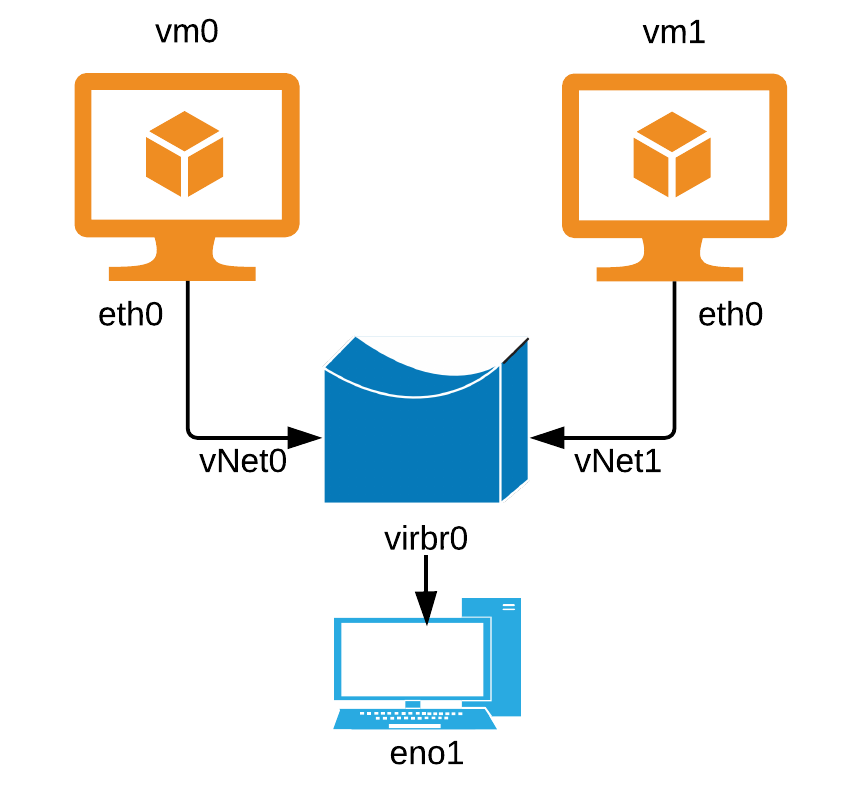
\includegraphics[width=0.5\linewidth]{Mod2/chapters/2.6.b}
	\caption{A virtualized network}
	\label{fig:2}
\end{figure}

\noindent	
The virtual bridge acts like a physical switch in the network and merely passes data between the networks. Note that it is incapable of routing decisions. All network traffic - even the traffic that originates from the physical KVM host are handled by it and thus, the virtual bridge decides who can send their packets at a specific moment. 

Each of the virtual machines have their own virtualized Ethernet interface called \verb|eth0| which have to be connected to an interface (port) on the virtual bridge. The virtual bridge names them \verb|vnet0| and \verb|vnet1| accordingly. 
\vspace{-10pt}

\subsection{Working with Network Bridges} \vspace{-10pt}
Let us consider a physical host with two KVM virtual machines running on it. Then, we can see their details using:

\vspace{-20pt}
\begin{minted}{console}
# virsh list --all
Id    Name                           State
----------------------------------------------------
3     vm0                            running
4     vm1                            running
\end{minted}
\vspace{-15pt}	

\noindent 
Linux has an inbuilt layer 2 Ethernet bridge. This can be controlled using the \verb|brctl| command. The status of the devices (VMs) connected to the bridge can be viewed with:

\vspace{-20pt}
\begin{minted}{console}
# brctl show
bridge name	 bridge id		STP enabled	interfaces
virbr0	      8000.525400683445	yes		virbr0-nic
								vnet0
								vnet1
\end{minted}
\vspace{-10pt}	

\noindent
The \verb|vnet0| and \verb|vnet1| interfaces are from the \verb|vm0| and \verb|vm1| virtual machines that are running on the host machine. The details of these interfaces can be seen with:

\vspace{-15pt}
\begin{minted}{console}
# ip link show
...
2: ens33: <BROADCAST,MULTICAST,UP,LOWER_UP> mtu 1500 qdisc pfifo_fast state UP mode DEFAULT qlen 1000
link/ether 00:0c:29:d8:97:c2 brd ff:ff:ff:ff:ff:ff
3: virbr0: <BROADCAST,MULTICAST,UP,LOWER_UP> mtu 1500 qdisc noqueue state UP mode DEFAULT qlen 1000
link/ether 52:54:00:68:34:45 brd ff:ff:ff:ff:ff:ff
...
7: vnet0: <BROADCAST,MULTICAST,UP,LOWER_UP> mtu 1500 qdisc pfifo_fast master virbr0 state UNKNOWN mode DEFAULT qlen 1000
link/ether fe:54:00:0d:4a:d5 brd ff:ff:ff:ff:ff:ff
8: vnet1: <BROADCAST,MULTICAST,UP,LOWER_UP> mtu 1500 qdisc pfifo_fast master virbr0 state UNKNOWN mode DEFAULT qlen 1000
link/ether fe:54:00:21:93:04 brd ff:ff:ff:ff:ff:ff
\end{minted}
\vspace{-10pt}	

\noindent
The virtual bridge \verb|virbr0| connects several devices together: the virtual ethernet interfaces from the VMs, \verb|vmnet0| and \verb|vmnet1| to the external LAN via interface \verb|ens33|, which is the NIC for the physical host. The virtual bridge only shows active interfaces connected to it, i.e., only when the VMs are running will they appear on the output of \verb|brctl show|. 

\subsection{Difference between network device and interface}
In terms of hardware, a device refers to the physical NIC that's connected to the host, while an interface refers to the physical port that an Ethernet cable is plugged into, i.e., the hardware Ethernet port. Back when each NIC had only one interface, the terms \textit{device} and \textit{hardware} meant the same thing. However, with the advent of NICs with multiple interfaces on the same NIC, for example dual or quad port configurations, interfaces refer to each separate hardware port that's capable of accepting a network cable. Thus, for a NIC with 4 hardware ports, the single device has 4 interfaces. 

Linux however, doesn't see these interfaces as connected devices (unless configured to do so) and treat them like separate hardware devices, even though they're on the same card! So, there can be multiple interfaces per hardware device. However, from Linux's perspective, they're all separate network devices, thus making the terms \textit{interface} and \textit{device} synonymous. 

\section{Setting up Network Bridges}
The roles of the interfaces on the bridge are defined by the connections (profiles) for the available interfaces. Thus, we generate new profiles for the interfaces that we want to act as slaves, and one connection for the interface that we intend to act as master.

\subsection{Creating a slave interface on the bridge}
The package needed to set up software bridges on RHEL 7 is called \verb|bridge-utils|. To set up bridging all connected interfaces need to be disconnected and then connected to the bridge. The connected interface can be viewed with:

\vspace{-15pt}
\begin{minted}{console}
# nmcli dev show
GENERAL.DEVICE:                         ens33
GENERAL.TYPE:                           ethernet
GENERAL.HWADDR:                         00:0C:29:3B:B9:1C
GENERAL.MTU:                            1500
GENERAL.STATE:                          100 (connected)
GENERAL.CONNECTION:                     ens33
GENERAL.CON-PATH:                       /org/freedesktop/NetworkManager/ActiveConnection/1
WIRED-PROPERTIES.CARRIER:               on
IP4.ADDRESS[1]:                         10.0.99.11/24
IP4.GATEWAY:                            10.0.99.2
IP4.DNS[1]:                             10.0.99.2
IP6.ADDRESS[1]:                         fe80::f408:1ebf:7742:9fd8/64
...
\end{minted}
\vspace{-10pt}	

\noindent
Now, we disconnect the devices using:

\vspace{-15pt}
\begin{minted}{console}
# nmcli dev disconnect ens33
Device 'ens33' successfully disconnected.
\end{minted}
\vspace{-10pt}	

\noindent
Once the disconnection is complete, we can now start defining the bridge, by adding an interface connection with:

\vspace{-15pt}
\begin{minted}{console}
# nmcli con add con-name br0-port1 type bridge-slave master br0 ifname ens33 
Warning: master='br0' doesn't refer to any existing profile.
Connection 'br0-port1' (3dee7b9b-6197-4eb7-be8d-46290361b9fd) successfully added.
\end{minted}
\vspace{-10pt}	

\noindent
In this command, we have created a new connection with the name \verb|br0-port1| and connected it to the interface \textit{ens33}, which refers to the hardware NIC of the host. We've set the connection type to \textbf{bridge-slave}, which refers to the fact that the details of the incoming connection to the \textit{slave} interface (\textit{ens33}) will be configured at the bridge. The master of the new slave connection is set to a connection called \textit{br0} (which doesn't yet exist, leading to the warnings).

The advantage of the master-slave configuration in network bridges is that if there are many connected slave interfaces, we need not set up their properties individually, and the master (bridge) thus provides a central point of configuration. The above slave configuration has to be repeated for every slave interface that we wish to connect to the bridge. 

\subsection{Creating a master interface on the bridge}
The connection for the master interface will determine the settings for all the slave interfaces connected to it. We create the master connection by setting the type to \verb|bridge| (instead of \verb|bridge-slave|, unlike the previous cases):

\vspace{-15pt}
\begin{minted}{console}
# nmcli con add con-name br0 type bridge ifname br0
Connection 'br0' (493c6288-7f40-4a9b-9ac0-aee7a7aebe71) successfully added.
# brctl show
bridge name	bridge id		STP enabled	interfaces
br0		8000.000000000000	yes			
\end{minted}
\vspace{-10pt}	

\noindent
The NetworkManager must be restarted to be actually able to use any of this, since these only refer to the configuration in scripts \verb|/etc/sysconfig/network-scripts| that need to be created by the NetworkManager. 

\vspace{-15pt}
\begin{minted}{console}
# cd /etc/sysconfig/network-scripts/
# ls ifcfg-*
ifcfg-br0  ifcfg-br0-1  ifcfg-br0-port1  ifcfg-ens33  ifcfg-lo
\end{minted}
\vspace{-10pt}	

\noindent
The contents of the interface configuration file for the br0 master port:

\vspace{-15pt}
\begin{minted}{bash}
DEVICE=br0
STP=yes
BRIDGING_OPTS=priority=32768
TYPE=Bridge
PROXY_METHOD=none
BROWSER_ONLY=no
BOOTPROTO=dhcp
DEFROUTE=yes
IPV4_FAILURE_FATAL=no
IPV6INIT=yes
IPV6_AUTOCONF=yes
IPV6_DEFROUTE=yes
IPV6_FAILURE_FATAL=no
IPV6_ADDR_GEN_MODE=stable-privacy
NAME=br0
UUID=5da1229d-27f1-4261-8491-e30046b9d03d
ONBOOT=yes
\end{minted}
\vspace{-10pt}	

\noindent
Since no information about IPs were provided, the boot protocol was chosen to be \textit{DHCP} automatically. The slave interfaces only have the configuration:

\vspace{-15pt}
\begin{minted}{bash}
TYPE=Ethernet
NAME=br0-port1
UUID=3dee7b9b-6197-4eb7-be8d-46290361b9fd
DEVICE=ens33
ONBOOT=yes
BRIDGE=br0
\end{minted}
\vspace{-10pt}	

\noindent
Since the configuration via the \verb|nmcli| utility is hard to remember, it's man page has a link to the \textit{nmcli-examples} man page, which has specific examples on setting up a bridge connection, as well as much more of the \verb|nmcli| functionality. 

	\section{Understanding Network Bonds and Teams}
Both network bonds and teams accomplish roughly the same goal - the aggregation of links or network interfaces to form Link Aggregation Groups (LAG) or virtual links. This means several physical/logical interfaces can be combined to form a \textit{team} that together fulfil a responsibility. Thus, one link may be set up as a primary connection to the WAN while the other may act as a backup or they both may be configured to act together while load balancing. Network bonding has been deprecated in RHEL 7 and thus we'll concentrate on Network teaming. 

Network bonding used to perform the same responsibility as network teaming, but in the user space. Contrastingly, network teaming works with a kernel driver but also has a user space daemon, called \textbf{teamd}. This \textit{teamd} daemon has several modes of operation called \textit{runners}. These determine the function of the ports in the team and have possible values of: \textit{broadcast, roundrobin, activebackup, loadbalance} and \textit{lacp}. 

\noindent
\begin{tabular}{rM{0.85}}
	\toprule
	\textbf{Terms} &\textbf{Description} \\
	\midrule
	\textbf{broadcast}	&Any packet is broadcast all over the interfaces.\\
	\midrule
	\textbf{roundrobin}	&The port which can transmit data is chosen in a roundrobin fashion.\\
	\midrule
	\textbf{activebackup}	&One of the interfaces stays active while the other is backup, ready to kick in the moment the active interface fails.\\
	\midrule
	\textbf{loadbalance}	&The network load (i.e., the packets in the network) is split between the interfaces so as to not overload any single interface.\\
	\midrule
	\textbf{lacp}	&Link Aggregation Control Protocol - allows formation of LAGs on a peer by automatically negotiating by transmitting LACP packets.\\
	\bottomrule
\end{tabular}

\noindent
The command to control and manage teams is called \verb|teamdctl|. Thus, to show the state of the team called \textit{team0}, we'd use: \verb|teamdctl team0 state|. 

	\section{Configuring Network Teams}
There are four parts to creating a team:
\begin{itemize}
	\item Creating a team interface
	\item Determining the network configuration
	\item Assigning the port interfaces
	\item Bring team and port interfaces up and down respectively. 
\end{itemize}

\noindent
Once the above has been taken care of, the team connection can be verified with \verb|teamdctl team0 status| (assuming \textit{team0} is the name of the team). 

\subsection{Creating the team interface}
We have to create the new team connection, preferably with the same interface name as the team:

\vspace{-15pt}
\begin{minted}{console}
# nmcli con add type team con-name team0 ifname team0 config '{"runner": {"name": "loadbalance"}}'
Connection 'team0' (d0eba200-591c-4ce3-a089-12d8a5692243) successfully added.
\end{minted}
\vspace{-10pt}	

\noindent
In this command, we have created a connection of type \textit{team}, which indicates that it'll be a link aggregate. We provide a name to it called \textit{team0} and connect it to an interface called team0 (which is logical - the interface that'll act as the aggregate of the member links). Finally, we provide the configuration as a JSON array: \verb|'{"runner": {"name": "loadbalance"}}'|. This sets the team to act as a load balancer, and thus split the load of the packets over all the interfaces configured in the team. 

\subsection{Determining the network configuration}
The team needs to be configured to use an IP address to use as its interface (i.e., team interface). This is specified using the CIDR (Classless Inter-Domain Routing) notation with a Network IP address and a prefix. From this both the Network ID and the Subnet mask can be determined. 

\vspace{-15pt}
\begin{minted}{console}
# nmcli con mod team0 ipv4.addresses 10.0.0.10/24
# nmcli con mod team0 ipv4.method manual
\end{minted}
\vspace{-10pt}	

\noindent
Note that the \verb|mod| command uses \verb|ipv4| instead of \verb|ip4|, unlike the \verb|nmcli add| command. The IP assignment method also needs to be switched to manual since DHCP isn't involved here. 

\subsection{Assigning the port interfaces}
Now that the master (team) interface has a port defined for it, we also need to assign the individual interfaces that are going to be slaves to the team. This is done using:

\vspace{-15pt}
\begin{minted}{console}
# nmcli con add type team-slave con-name team0-ens33 ifname ens33 master team0
Connection 'team0-ens33' (78e706bd-395c-456f-b16a-75430c48be2c) successfully added.
# nmcli con add type team-slave con-name team0-enss37 ifname ens37 master team0
Connection 'team0-enss37' (d17ad2f5-9a55-422a-ad5d-f4b327674393) successfully added.
\end{minted}
\vspace{-10pt}	

\noindent
The command defines two interfaces (\textit{eth0} and \textit{eth1}) to be slaves to the team interface. They are named according to the format \verb|<teamName>-<interfaceName>|. Now we only need to define a master for them from which they can be controlled. 

\subsection{Bringing the team and port interfaces up/down}
Once the above sections have been handled, the team is basically ready for operation. However, we still need to bring the physical devices (that are slaves to the team) to be disconnected and then reconnected as part of the team. Since we've already defined them as a part of the team, we just need to:

\vspace{-15pt}
\begin{minted}{console}
# nmcli con up team0
Connection successfully activated (master waiting for slaves) (D-Bus active path: /org/freedesktop/NetworkManager/ActiveConnection/7)
# nmcli dev disconnect ens33; nmcli dev dis ens37
Device 'ens33' successfully disconnected.
Device 'ens37' successfully disconnected.
\end{minted}
\vspace{-10pt}	

\noindent
The devices \textit{eth0} and \textit{eth1} needed to be disconnected because they're slaves to the team now, and thus, their operation should only be influenced by the team itself. Thus, there's no point in having them exist as separate individual devices (network interfaces). 

\subsection{Verifying the team connection}
We can verify the team connection by:
\vspace{-15pt}
\begin{minted}{console}
# teamdctl team0 state
setup:
  runner: loadbalance
ports:
  ens33
    link watches:
      link summary: up
      instance[link_watch_0]:
        name: ethtool
        link: up
        down count: 0
  ens37
    link watches:
      link summary: up
      instance[link_watch_0]:
        name: ethtool
        link: up
        down count: 0
\end{minted}
\vspace{-10pt}	

\subsection{Creating a bridge based on Network Teams}
When creating bridges based on network teams, it becomes important to switch off NetworkManager since they're incompatible. The team configuration file \verb|ifcfg-team0| needs to be edited to add the line \verb|BRIDGE=brteam0| has to be added to it to ask it to connect to the bridge device. 

Since the team interfaces will be slaves to the connection provided by the team, it's important to ensure that there are no IP configurations in the \verb|ifcfg-team0-port| files anymore. Basically, we need to disable the team driver since the bridge will now control the team interface. For this we do:

\vspace{-15pt}
\begin{minted}{console}
# nmcli dev dis team0
# systemctl stop NetworkManager; systemctl disable NetworkManager
\end{minted}
\vspace{-10pt}	

\noindent


Now we can manually create a configuration file for the bridge connection that has the contents:

\vspace{-15pt}
\begin{minted}{bash}
DEVICE=brteam0
TYPE=Bridge
IPADDR0=192.168.122.100
PREFIX0=24
\end{minted}
\vspace{-10pt}	

\noindent
Finally, since we're not using the \verb|NetworkManager| service, we directly restart the networking with: \verb|systemctl restart network|. Now, the bridge on top of the team interface should be active and operational. Again, examples for these congigurations are present in the nmcli-examples man page, accessible with \verb|man 5 nmcli-settings|. 

\section{Configuring IPv6} 
Since there is a shortage of unique IPv4 addresses when compared to the number of devices that are connected to the internet, IPv6 is the new standard for the IP addresses. Just like IPv4 addresses, it can be divided into two parts: the network ID and the host ID. However, in the case of the IPv6 addresses, the host ID contains the MAC address of the interface itself! A typical IPv6 address looks like:

\vspace{-15pt}
\begin{minted}{bash}
fe80::2af4:9908:7092:34cb/64
\end{minted}
\vspace{-10pt}	

\noindent
In this, the network ID is \verb|fe80| while the node part is the \verb|2af4:9908:7092:34cb| with the prefix of \verb|64| defining how long the network ID is. Thus, the computer listens for the Network ID, and then appends it's own MAC address to obtain a truly unique IPv6 address! For configuring connections with both IPv6 and IPv4 addresses, nmcli can be used as:

\vspace{-15pt}
\begin{minted}{console}
# nmcli con add con-name testCon type ethernet ip6 2001:db8:0:10::d000:310/64 gw6 2001:db8:0:10::1 ip4 192.168.0.10/24 gw4 192.168.0.1
\end{minted}
\vspace{-10pt}	

\noindent
Again, for new connection just like for IPv4 connections where \verb|nmcli con add| takes as argument the term \textbf{ip4} instead of \textit{ipv4} (unlike the \verb|con mod| command, which accepts \textit{ipv4}), the \verb|nmcli con add| needs an argument of \textbf{ip6} and not \textit{ipv6}. Now to add a DNS server for it:

\vspace{-15pt}
\begin{minted}{console}
# nmcli con mod testCon +ipv6.dns 2001:4680:4680::8888
\end{minted}
\vspace{-10pt}